\documentclass[crop,tikz]{standalone}

\usepackage{fontspec}
\setmainfont{texgyrepagella}[
  Extension = .otf,
  UprightFont = *-regular,
  BoldFont = *-bold,
  ItalicFont = *-italic,
  BoldItalicFont = *-bolditalic,
]

\usepackage{tikz}
\usetikzlibrary{decorations.pathreplacing,calligraphy}
\usetikzlibrary{calc}

\makeatletter % https://tex.stackexchange.com/a/38995/121799
\tikzset{
  use path/.code={\pgfsyssoftpath@setcurrentpath{#1}}
}
\makeatother
\tikzset{reverseclip/.style={insert path={(current bounding box.north
        east) rectangle (current bounding box.south west)}}}

\pgfdeclarelayer{bg}
\pgfsetlayers{bg,main}


\begin{document}
    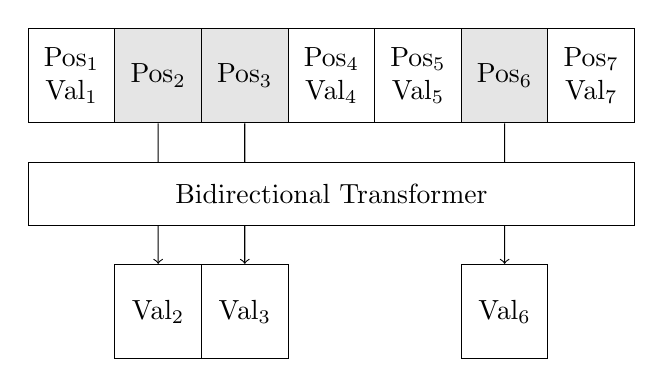
\begin{tikzpicture}

        \tikzstyle{every node}=[draw,rectangle, minimum width=1.1cm,anchor=west,align=center]

        \foreach \i / \x in {0/1,3/4,4/5,6/7} {
            \node[text width=0.8cm, minimum height=1.2cm] (i_\x) at (\i*1.1cm, 0) {Pos$_{\x}$ Val$_{\x}$};
        }
        \foreach \i / \x in {1/2,2/3,5/6} {
            \node[text width=0.8cm, minimum height=1.2cm,fill=white!90!black] (i_\x) at (\i*1.1, 0) {Pos$_{\x}$};
            \node[text width=0.8cm, minimum height=1.2cm] (t_\x) at (\i*1.1 cm, -3cm) {Val$_{\x}$};

            \begin{pgfonlayer}{bg}
                \draw[->] (i_\x) -- (t_\x);
            \end{pgfonlayer}
        }

        \node[minimum width=1.1cm*7,fill=white, minimum height=0.8cm] (transformer) at (0, -1.5cm) {Bidirectional Transformer};



    \end{tikzpicture}
\end{document}
